Türkiye Burslari Scholarships (YTB) adalah beasiswa untuk program S1, S2, S3, penelitian, dan program Bahasa Turki untuk mahasiswa internasional. Apa saja beasiswa yang ditawarkan? Berikut informasi selengkapnya dari Schoters.
\begin{figure}[!htbp]
	\centerline{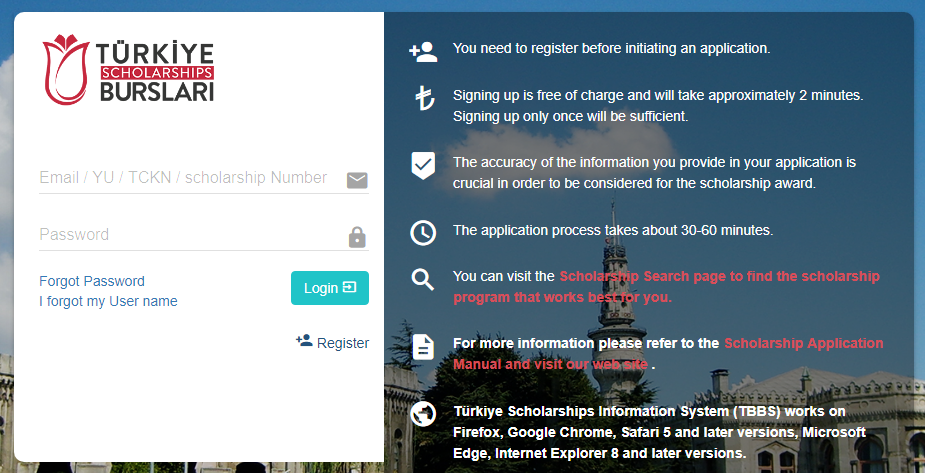
\includegraphics[width=0.75\textwidth]{figures/1/main_page.PNG}}
	\caption{Halaman Utama Turkiye Burslari Scholarship}
	\label{fig1:main_page}
\end{figure}

\section{Jenis-Jenis Beasiswa YTB}

\subsection{Daftar Beasiswa Türkiye Burslari untuk Program Sarjana}

\begin{enumerate}
\item Bosphorus Undergraduate Scholarship Program

Bosphorus Undergraduate Scholarship Program adalah beasiswa yang diberikan untuk calon mahasiswa sarjana dari berbagai negara, salah satunya Indonesia. Program beasiswa ini memberi kesempatan kepada calon mahasiswa untuk menempuh pendidikan di semua program sarjana di Turki, selain jurusan kedokteran, agama, sastra dan bahasa turki.

\item Anatolian Undergraduate Scholarship Program

Anatolian Undergraduate Scholarship Program adalah beasiswa yang diberikan untuk pelajar asing yang telah menempuh pendidikan SMA di Turki. Mereka yang berminat untuk melanjutkan sekolah di universitas di Turki boleh melamar beasiswa ini. Calon mahasiswa boleh memilih kuliah di jurusan apa saja, selain jurusan kedokteran, agama, sastra dan bahasa turki.
\end{enumerate}

\subsection{Daftar Beasiswa Türkiye Burslari untuk Program Master dan Doktor}

\begin{enumerate}
\item Ali Kuşçu Science and Technology Graduate Scholarship

Ali Kuşçu Science and Technology Graduate Scholarship program adalah beasiswa yang diberikan untuk lulusan S1 dan S2 yang ingin melanjutkan studi ke Turki dalam bidang Science dan Engineering and Technology. Beasiswa ini dibuka untuk seluruh mahasiswa internasional dari seluruh negara.

\item İbni Haldun Social Sciences Graduate Scholarship

İbni Haldun Social Sciences Graduate Scholarship adalah beasiswa yang diberikan untuk calon mahasiswa yang ingin mengambil program Master dan Doktor di bidang Social Science. Program beasiswa ini juga terbuka untuk seluruh kandidat dari seluruh negara.
\end{enumerate}

\subsection{Daftar Beasiswa Türkiye Burslari untuk Program Aplikasi Jurusan Tertentu}

\begin{enumerate}
\item İbni Sina Medical Sciences Scholarship Program

İbni Sina Medical Sciences Scholarship adalah beasiswa yang diberikan untuk calon mahasiswa internasional yang ingin melanjutkan studi pada bidang kedokteran, kedokteran gigi, farmasi, dan kedokteran hewan. Beasiswa ini diperuntukkan untuk program Associate, Undergraduate, Master’s degree, dan PhD degree. Program ini terbuka untuk seluruh mahasiswa asing dari seluruh negara.

\item Yunus Emre Turkish Language Scholarship Program

Yunus Emre Turkish Language Scholarship memberikan beasiswa kepada calon mahasiswa internasional yang ingin mempelajari Bahasa Turki di Turki. Beasiswa ini diperuntukkan untuk mahasiswa program Sarjana, Master, dan Doktor. Program ini terbuka untuk seluruh mahasiswa asing dari seluruh negara

\item Islamic Studies Scholarship Program

Islamic Studies Scholarship program adalah beasiswa yang diberikan untuk mahasiswa program Sarjana, Master, dan Doktor yang ingin mempelajari bidang agama di Turki. Beasiswa ini terbuka untuk seluruh mahasiswa asing dari seluruh negara.
\end{enumerate}
 
\subsection{Daftar Beasiswa Türkiye Burslari untuk Program Jangka Pendek}

\begin{enumerate} 
\item Support and Succes Scholarship Program

Support and Success Scholarship Program adalah beasiswa yang diberikan untuk mahasiswa internasional yang sedang belajar di universitas di Turki

\item Research Scholarships

Research Scholarships oleh Türkiye Burslari adalah beasiswa yang diberikan untuk mahasiswa program Doktor yang berasal dari luar Turki. Untuk mendaftar beasiswa ini, kandidat harus diterima di salah satu universitas di Turki. Penelitian akan dilaksanakan jika memenuhi kriteria bahasa di universitas tersebut.
\end{enumerate}

\subsection{Daftar Beasiswa Türkiye Burslari untuk Program Pendidikan Bahasa dan Budaya Turki}

Program beasiswa ini ditujukan untuk para pejabat publik, diplomat, akademisi, dan peneliti yang ingin mempelajari bahasa dan kebudayaan Turki. Beasiswa ini dibuka untuk umum dan pendaftarannya dilakukan melalui Kedutaan Besar Turki di negara masing-masing. Beasiswa ini mencakup gaji bulanan dan biaya asrama. Kandidat akan mengikuti program selama 8-10 bulan.

\section{Cakupan Beasiswa}

\begin{enumerate}
\item Uang saku/bulan S1= 700TL, S2= 950TL, S3 = 1400 TL dan penelitian 3000 TL. Sedangkan Program Jangka Pendek S1= 440 TL, S2= 590 TL dan S3=  880TL. (Catatan:  Program jangka pendek dan penelitian tidak mencakup akomodasi dan lain sebagainya)
\item Asrama gratis. Bagi pelamar S2 atau S3 yang sudah menikah, biaya asrama akan diganti dengan tunjangan tempat tinggal sebesar 500 TL.
\item Biaya pendidikan. Termasuk kuliah musim panas atau mengambil kuliah di Universitas lain di Turki.
\item Biaya Kesehatan. Biaya Pengobatan gratis di rumah sakit pemerintah dan diskon di rumah sakit swasta.
\item Kursus Bahasa Turki.
\item Tiket Pesawat. Terdiri dari tiket keberangkatan pertama dan setelah lulus
\end{enumerate}

\section{Kriteria Penerima Beasiswa}

\begin{enumerate}
\item Umur maksimal bagi pendaftar beasiswa TBS yaitu:
\begin{itemize}
\item Tidak lebih dari 21 tahun bagi yang berniat mendaftar untuk jenjang s1
\item Tidak lebih dari 30 tahun bagi yang berniat mendaftar untuk jenjang s2
\item Tidak lebih dari 35 tahun bagi yang berniat mendaftar untuk jenjang s3
\item Tidak lebih dari 45 tahun bagi yang berniat mendaftar beasiswa penelitian.
\end{itemize}
\item Nilai minimum untuk masing-masing jenis program dan beasiswa berbeda satu sama lain..
\begin{itemize}
\item Bagi pendaftar jenjang pendidikan sarjana s1, nilai minimum ijasah pendidikan sebelumnya 70 dari 100.
\item Bagi pendaftar jenjang master dan doctoral, nilai minimum ijasah pendidikan sebelumnya 75 dari 100.
\item Bagi pendaftar jurusan kedokteran, nilai minimum ijasah pendidikan sebelumnya 90 dari 100.
\end{itemize}
\item Pendaftar dapat berasal dari seluruh negara di dunia
\item Status pendaftar: sudah lulus atau akan lulus sebelum September 2019
\item Bukan warga negara Turki atau sudah terdaftar di Universitas yang ada di Turki
\end{enumerate}

\section{Persyaratan Dokumen}
\begin{enumerate}
\item Nilai Ijazah/Surat Keterangan Lulus. Jika belum lulus, di fomulir online YTB silahkan diisi belum lulus atau sedang dalam periode penelitian.
\item Transkrip nilai/Rapor. Transkrip sementara atau rapor dapat digunakan jika belum lulus.
\item Ujian seleksi masuk universitas di Turki (jika ada)
\item Sertifikat/Penghargaan. Kumpulkan semua prestai yang pernah diraih.
\item Sertifikat Ujian Internasional seperti TOEFL, IELTS, GRE/GMAT (jika ada)
\item Kartu tanda pengenal seperti KTP/Paspor dan Kartu Keluarga
\item Mengisi essai yang ada di fomulir online YTB
\item Mengisi fomulir online YTB dengan lengkap. Jangan sampai ada keterangan berwarna merah pada sub menu fomulir online.
\end{enumerate}

\section{Proses Pendaftaran}

Pendaftaran beasiswa Türkiye Burslari Scholarships dilakukan dengan cara mengisi formulir pendaftaran online .

\section{Deadline Pendaftaran}

Pendaftaran Türkiye Burslari Scholarships ditutup pada tanggal 24 Februari 2019. Kandidat akan diseleksi berdasarkan keberhasilan di bidang akademik dan juga hasil dari wawancara. Kriteria pendidikan dari setiap kandidat akan ditentukan berdasarkan nilai-nilai yang tercantum pada dokumen-dokumen persyaratan pendaftaran beasiswa YTB.

Informasi lebih lanjut tentang Türkiye Burslari Scholarships bisa dilihat https://turkiyeburslari.gov.tr


